\section{Introduction}
\label{sec:introduction}

The fine-grained data annotation capabilities provided by key-value storage is
a natural match for many types of scientific simulation. In simulations relying
on the finite element method, a mesh-based decomposition of a physical region,
may result in millions or billions of mesh cells each containing materials,
pressures, temperatures and other characteristics that are required to
accurately simulate phenomena of interest. In our target application, the
ParSplice~\cite{perez:jctc20150parsplice} molecular dynamics simulation, a
hierarchy of cache nodes and a single node key-value store are used to store
both observed minima across a molecule's equation of motion (EOM) and the
hundreds or thousands of partial trajectories calculated each second during a
parallel job. Unfortunately, if we scale the system the IO to the storage
hierarchy will quickly saturate both the storage and bandwidth capacity of a
single node. 

\begin{figure}[t]
  \noindent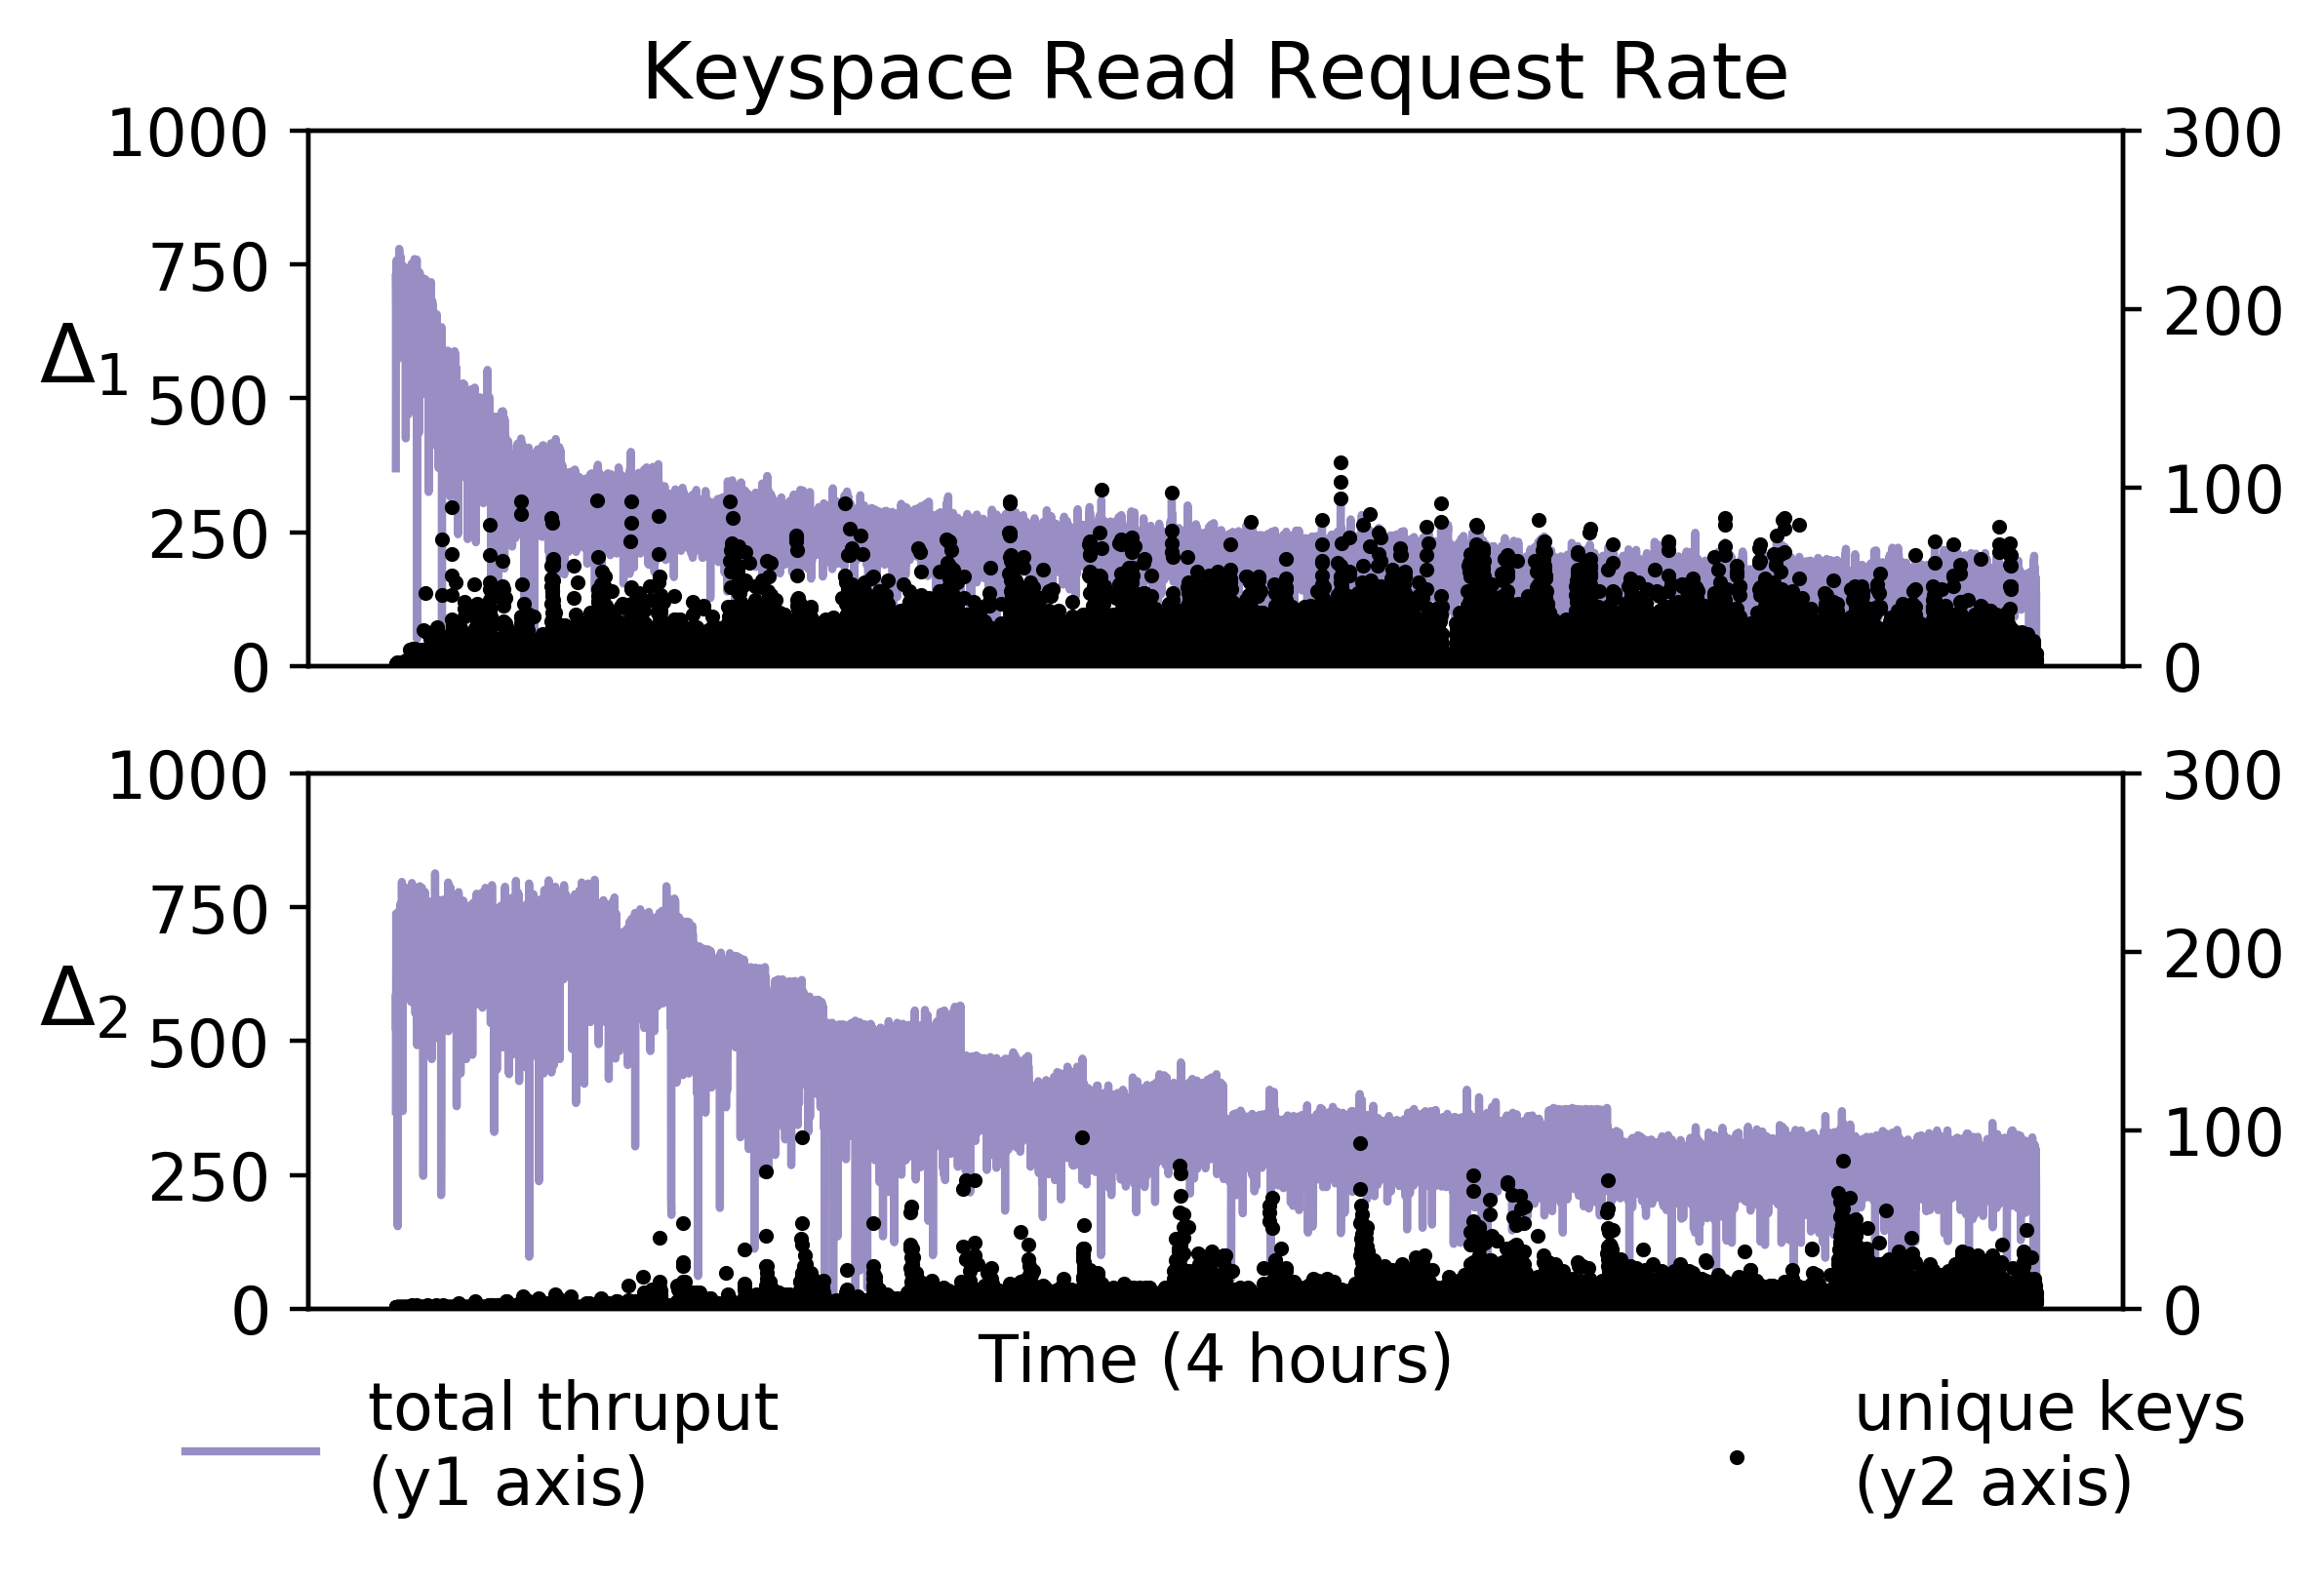
\includegraphics[width=0.4\textwidth]{figures/motivation-regimes.png}\\
  \caption{The keyspace activity for ParSplice runs using two different growth
  rates.  The line shows the rate at which EOM minima values are retrieved
  from the key-value store (\(y1\) axis) and the scattered points along the
  bottom show the number of unique minima keys accessed in a 1 second sliding
  window (\(y2\) axis).  \label{fig:motivation-regimes}}
\end{figure}


To motivate the need for load balancing data across a distributed key-value store,
we show how limiting the cache size saves memory and sacrifices negligible
performance. This type of analysis will help inform our load balancing policies
for when we switch to a distributed key-value store back-end to store segment
coordinates.  We need to know when and how to partition the keyspace: a smaller
cache hurts performance because key-value pairs need to be retrieved from other
nodes while a larger cache has higher memory usage. 

In this paper we present a detailed analysis of how the ParSplice application
accesses EOM minima key-value pairs over the course of a long running simulation
across a variety of initial conditions. Figure~\ref{fig:motivation-regimes}
shows that small changes to the rates at which new atoms enter the simulation,
or the initial temperature at which the simulation begins can have a strong
effect on the timing and frequency with which new EOM minima are discovered and
referenced.

We also demonstrate the Mantle~\cite{sevilla:sc15-mantle} approach to load
balancing for software-defined storage systems.  Although Mantle was initially
developed for the Ceph distributed file system, the flexible policy-based
approach to load balancing provided by Mantle is also applicable to the
changing key-value workloads generated by ParSplice. The Mantle load-balancing
API enables the storage system to change the active load-balancing policy in
use, a technique we will show is critical in applications such as ParSplice
that have alternating stable and chaotic simulation ``access regimes" over the
course of a long-running simulation.  Effectively, Mantle provides us the
ability to choose among several load-balancing policies as needed.

Finally, we explore the use of simple machine learning (ML) techniques to
identify access regimes within the ParSplice application's creation and access
of key-value pairs. The ML component of this work drives the Mantle
policy-switching API and helps determine \emph{when} and \emph{how} to change
policies.

By understanding the regime-based key-value access patterns generated by
ParSplice, leveraging the dynamic load balancing capabilities of the Mantle
API, and using ML to identify key-value access regime changes we are working
toward a flexible load balancing capability for software-defined storage
systems. 
